\section{Einleitung}
Ein beliebtes regelungstechnisches Problem ist die Regelung eines inversen Pendels an einem Wagen (Abb. \ref{fig:wp}). Die Voraussetzung dafür ist das Vorhandensein eines guten Systemmodells. Während solche Modelle berechnet werden können \cite[Softwarebeispiel 3]{Knoll2016}, soll hier untersucht werden, ob ähnliche Ergebnisse mit SINDy reproduziert werden können, oder ob SINDy zur Parameterschätzung genutzt werden kann. 
\begin{figure}[h!] %wp
	\centering
	\includegraphics[width=75mm]{images/wp.jpg}
	\caption{Schematische Darstellung des Wagen-Pendel-Systems, mit den Massen $m_1$ und $m_2$, der Pendellänge $s$, der Erdbeschleunigung $g$, dem Krafteingang $F$, der Position des Wagens $x$ und der Auslenkung des Pendels aus der unteren Ruhelage $\varphi$.}
	\label{fig:wp}
\end{figure}
Das Wagen-Pendel-System wird durch folgende DGL beschrieben:
\begin{align}
	\dot{\boldsymbol{x}} &= \begin{pmatrix}
		\dot{x_1}  \\
		\dot{x_2}  \\
		\dot{x_3}  \\ 
		\dot{x_4}	
	\end{pmatrix} 	=	\begin{pmatrix}
							\dot{\varphi} \\
							\dot{x}  \\
							\ddot{\varphi}  \\ 
							\ddot{x}
						\end{pmatrix} = f(\boldsymbol{x}) + g(\boldsymbol{x}) u\\
	&=\begin{pmatrix}
		\dot{\varphi}  \\
		\dot{x}  \\
		-\frac{m_2s\dot{\varphi}^2\sin\varphi\cos\varphi + (m_1+m_2)g\sin\varphi}{s(m_1 + m_2\sin^2\varphi)}\\
		\frac{gm_2\sin\varphi\cos\varphi + m_2s\dot{\varphi}^2\sin\varphi}{(m_1+m_2\sin^2\varphi)}   
	\end{pmatrix}		
 +		 \begin{pmatrix}
									0  \\
									0  \\
									-\frac{\cos\varphi}{s(m_1 + m_2\sin^2\varphi)}\\
									\frac{1}{m_1+m_2\sin^2\varphi}   
								\end{pmatrix} F. \label{eq:wp}
\end{align}
Der Einfachheit halber wird nur das autonome System betrachtet, daher gilt $F\equiv0$. 
Ausgehend von den zeitlichen Verläufen der Zustandskomponenten und deren Ableitungen sollen die Struktur und die Parameter $\boldsymbol{p}=\begin{pmatrix*}[c] m_1& m_2& s & g \end{pmatrix*}$ des Systems bestimmt werden.

\section{Aufbau der Bibliothek}
\label{sec:aufbauderbibo}
Das Wagen-Pendel-System wird im Gegensatz zu den bisher betrachteten Systemen nicht ausschließlich durch Polynome beschrieben. Das macht die Konstruktion der Bibliothek deutlich schwieriger. Der Algorithmus berechnet eine Linearkombination von Ansatzfunktionen, die das System modellieren sollen. Schreibt man die letzten beiden Zeilen von \eqref{eq:wp} als Summe
\begin{equation}
	\begin{pmatrix}
		\ddot{\varphi}  \\
		\ddot{x}  	
	\end{pmatrix}
	=\begin{pmatrix}
		-\frac{m_2s\dot{\varphi}^2\sin\varphi\cos\varphi}{sm_1 + sm_2\sin^2\varphi} - \frac{(m_1+m_2)g\sin\varphi}{sm_1 + sm_2\sin^2\varphi}\\
		\frac{gm_2\sin\varphi\cos\varphi}{m_1+m_2\sin^2\varphi} + \frac{m_2s\dot{\varphi}^2\sin\varphi}{m_1+m_2\sin^2\varphi}  , 
	\end{pmatrix}		
\end{equation}
so fällt auf, dass in jeder Zeile nur zwei verschiedene Ansatzfunktionen vorkommen. Diese müssen dem Algorithmus in der Bibliothek vorgegeben werden. Es lohnt sich darauf hinzuweisen, dass es nicht ausreicht, eine Bibliothek aus den vorkommenden Elementarfunktionen ($\sin, \cos$, Zustandskomponenten, Identität) anzulegen in der Hoffnung, dass SINDy diese geeignet verknüpft. SINDy kann die vorgegeben Funktionen nur additiv durch die angesprochene Linearkombination verknüpfen. 
Damit eine Identifikation möglich ist, muss sich jede Zeile der DGL wie folgt aus Funktionen $u_i$ und $v_i$ darstellen lassen:
\begin{equation}
x_i=\sum_{k}u_k(\boldsymbol{p})v_k(\boldsymbol{x}), \label{eq:right_side_decomp}
\end{equation}
wobei $u_i$ nicht von $\boldsymbol{x}$ und $v_i$ nicht von $\boldsymbol{p}$ abhängig sein darf. Dies ist auf Grund der Struktur der Nenner hier nicht möglich. Daher müssen die Nenner in diesem Beispiel als bekannt vorausgesetzt werden. 
Die Zähler haben eine für die Identifikation günstige Struktur, da sie Bedingung \eqref{eq:right_side_decomp} erfüllen. Dabei werden maximal vier Elementarfunktionen miteinander multipliziert. Um die Bibliothek systematisch aufzubauen, müssten für die Zähler alle Kombinationen mit Wiederholung aus maximal vier Elementarfunktionen berücksichtigt werden. Damit ergeben sich $C^r(13,4) = 1820$\footnote{Es gibt 13 mögliche Faktoren: $\sin$ und $\cos$ von jeder Zustandskomponente, vier Zustandskomponenten, Identität.} mögliche Zähler, wodurch die Bibliothek viel zu groß ist. Um das zu verhindern müssen einschränkende Annahmen getroffen werden:
\begin{itemize}
\item Nur die Auslenkung des Pendels aus der unteren Ruhelage $\varphi$ darf als Argument der Winkelfunktionen verwendet werden. 
\item Nur $\dot{\varphi}$ kann außerhalb der Winkelfunktionen vorkommen.
\end{itemize}
Damit verringert sich die Anzahl an möglichen Zählern auf $C^r(4,4) = 35$. Aus diesen Zählern und den bekannten Nennern kann der Großteil der Ansatzfunktionen für die Bibliothek erzeugt werden. Es fehlen nur noch Monome ersten Grades, um die ersten beiden Zeilen der DGL abbilden zu können. Damit ergibt sich eine Bibliothek aus 39 Ansatzfunktionen. Jedoch liefert diese noch nicht das gewünschte Ergebnis. Problematisch ist, dass es in der Bibliothek linear abhängige Spalten gibt, da gilt: 
\begin{equation}
\cos \varphi = \cos ^3 \varphi+ \sin^2 \varphi\cos \varphi.
\end{equation}
Dadurch kann, statt der vollständig vereinfachten Gleichung, eine zwar mathematisch richtige, jedoch wenig verwertbare Gleichung geliefert werden, da diese erst vereinfacht und die Koeffizienten neu berechnet werden müssten. Stattdessen kann man die Bibliothek noch einmal verkleinern, indem man die linear abhängigen Spalten entfernt. Diese kann man finden, indem man den Spaltenrang der ersten $i$ Spalten mit dem Spaltenrang der ersten $i+1$ Spalten der Bibliothek vergleicht. Sind die Ränge gleich, ist die $i+1$-te Spalte von den ersten $i$ Spalten linear abhängig und kann entfernt werden. Führt man diesen Prozess für die gesamte Bibliothek aus, so bleiben am Ende noch 28 Ansatzfunktionen übrig\footnote{Die Auswahl der 28 Spalten ist nicht eindeutig, aber mathematisch äquivalent, da die resultierenden Gleichungen gegebenenfalls vereinfacht werden können.}. Die Bibliotheksmatrix besitzt vollen Rang.

\section{Bewertung der Ergebnisse}
Unter Nutzung des Wissens über die geeignete Wahl der Identifikationsparameter und Verwendung mehrerer Trajektorien ist die Identifikation, wie in Abb. \ref{fig:sim_wp} ersichtlich, erfolgreich.
\begin{figure}[h!] %sim
	\centering
	\begin{subfigure}{.5\textwidth}
	  \centering
	  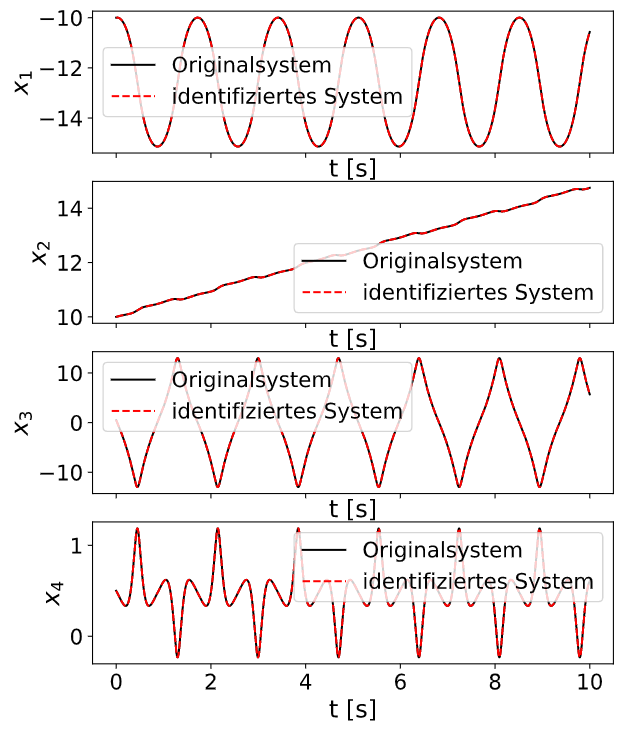
\includegraphics[width=75mm]{images/sim_wp_sim.png}
	  \caption{Simulationsverlauf}
	  \label{fig:sim_wp_sim}
	\end{subfigure}%
	\begin{subfigure}{.5\textwidth}
	  \centering
	  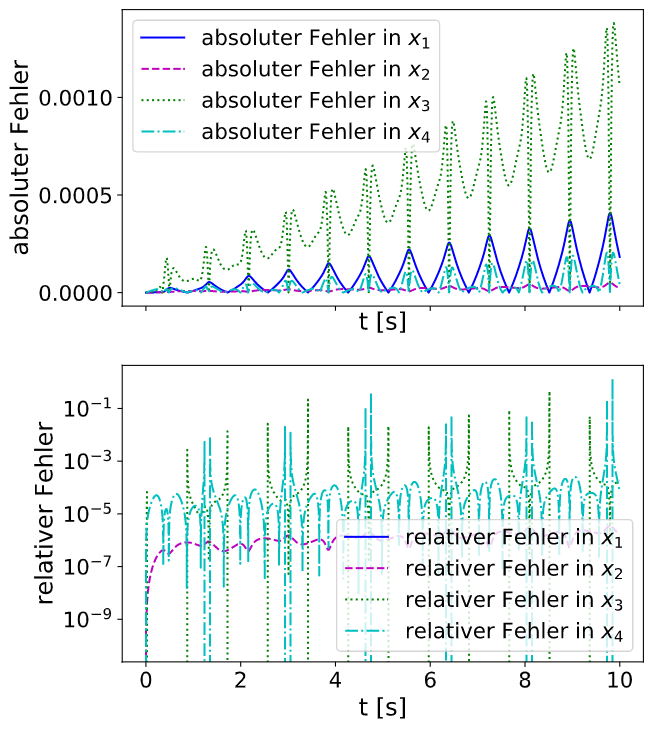
\includegraphics[width=75mm]{images/sim_wp_err.png}
	  \caption{Fehlerverlauf}
	  \label{fig:sim_wp_err}
	\end{subfigure}
	\caption{Simulation des Wagen-Pendel-Systems, relativer Fehler der identifizierten Koeffizienten $\varepsilon_\text{r} = 8\cdot 10^{-5}$.}
	\label{fig:sim_wp}
\end{figure}
Auf Grund der komplexen Struktur des Wagen-Pendel-Systems ist der SINDy-Algorithmus ohne beträchtliches Vorwissen über das System und einige Vereinfachungen nicht geeignet. Lassen sich die Differentialgleichungen nicht als Linearkombination relativ einfacher Funktionen darstellen, stößt die Methode schnell an ihre Grenzen. Allerdings zeigt das Beispiel, dass SINDy sehr gute Ergebnisse liefern kann, wenn die Struktur des Systems bereits bekannt ist und nur Parameter geschätzt werden sollen. 







